%!TEX root = ../thesis.tex

\chapter{Numerical Methods}
\label{chapter:methods}
\thispagestyle{myheadings}

% set this to the location of the figures for this chapter. it may
% also want to be ../Figures/2_Body/ or something. make sure that
% it has a trailing directory separator (i.e., '/')!
\graphicspath{{Numerical_Methods/}}

%%%%% METHODS

This section describes in detail the exact numerical methods used in this thesis, along with relevant formulae and implementation details. We start by discussing the different types of numerical integrals that will be used, including analytical and semi-analytical routines for singular integrals. Finally, we provide details about the relaxation schemes that will form the basis of our experimentation, along with preconditioners that will be used along with and in competition to relaxation schemes.


%and which equations we will use for testing purposes. For each of the two example equations we experiment with, we derive the {\bem} formulation, as well as introduce the expansions used for the {\fmm}. Then, the treatment of integrals within {\bem} is discussed, including singular integrals with analytical and semi-analytical methods. Finally we provide details about the relaxation strategies and preconditioners we will use throughout our numerical experimentation.

%To experiment with all of the different components described in \S\ref{sec:background}, we have a brand-new {\fmm} code written from the ground up to be extensible, easy to use and simple to integrate into larger applications.
%
%The code is written in {\cpp}, extensively using {\cpp}11 features, using templates to provide  delineated components, such that any one component can be changed, and as long as it complies with a fixed interface, no other code need be changed. The major components are:
%
%\begin{enumerate}
%	\item \emph{Tree Structure} -- Decompose the domain into boxes, only needs to offer an interface to the boxes, the particles contained within leaf nodes, and the ability to query the connectivity between boxes (children and parents).
%	\item \emph{Evaluator} -- This is responsible for traversing the tree, and dictating exactly which operators are called, and in what order. For example, treecodes and {\fmm}s would merely have differing evaluators.
%	\item \emph{Kernel} -- This implements all of the needed operators for treecodes and/or FMMs. A minimal kernel need only have {\ptop}, {\ptom}, {\mtom} and {\mtop} operators (treecode). Further, we offer the ability to provide either serial or vectorized versions of operators -- for instance, a {\ptop} operation could be defined as point vs. point, or box vs. box. This allows  optimized kernels to be used if preferred, but lowers the initial cost of implementation.\end{enumerate}


%%%%%%%%%%%%%%%%%%%%%%%%%%%%
% STOKES
%%%%%%%%%%%%%%%%%%%%%%%%%%%%


%%%%% NUMERICAL INTEGRATION
\section{Numerical Integration}\label{subsec:numerical_integration}

For all the {\bem} formulations described in this work, we must integrate some function, $f(\vect{x},\vect{y})$ over a source panel, $\Gamma,\;\vect{y}\in\Gamma$ with respect to a target point, $\vect{x}$ in order to generate a matrix element. This section deals with how to perform these integrals with sources and targets in different parts of the domain.

\begin{equation}
	\int_\Gamma f(\vect{x},\vect{y})\;\di{\Gamma}.
\end{equation}

We can separate the types of integrals we need to perform in terms of the distance between the source panel and target point. We introduce the following terms to describe this separation:

\begin{itemize}

\item \emph{Far} -- Integrals where the source and target panels are far apart require much less accuracy than either of the 2 other categories. In order to accelerate the far-field evaluation for an {\fmm}, semi-analytical and analytical integrals are unsuitable, and in these cases, Gauss quadrature rules of low order ($\{1, 3, 4, 7\}$ quadrature points) are sufficient, fast, and suitable for acceleration using an {\fmm}.

\item \emph{Near-singular} -- This kind of integral occurs when the source panel and target point are close-by (defined somewhat arbitrarily), but not the same. The integral is non-singular, but still requires high accuracy.  High-precision versions of standard quadrature rules are suitable in these cases, or the analytical / semi-analytical methods developed for singular integrals can be re-used.

\item \emph{Singular} -- The integral of a singular function over a region that includes a singularity. In the case of {\bem}, this occurs when the target point is within the source panel. Due to the singularity, most standard approximation techniques cannot be used, and so special methods must be developed, such as analytical or semi-analytical integrals.
	
\end{itemize}

The domain for each of these methods is shown graphically in figure \ref{fig:integration_domain}, and methods for each along with an implemented example are described in the following sections.

\begin{figure}[h]
	\begin{centering}
	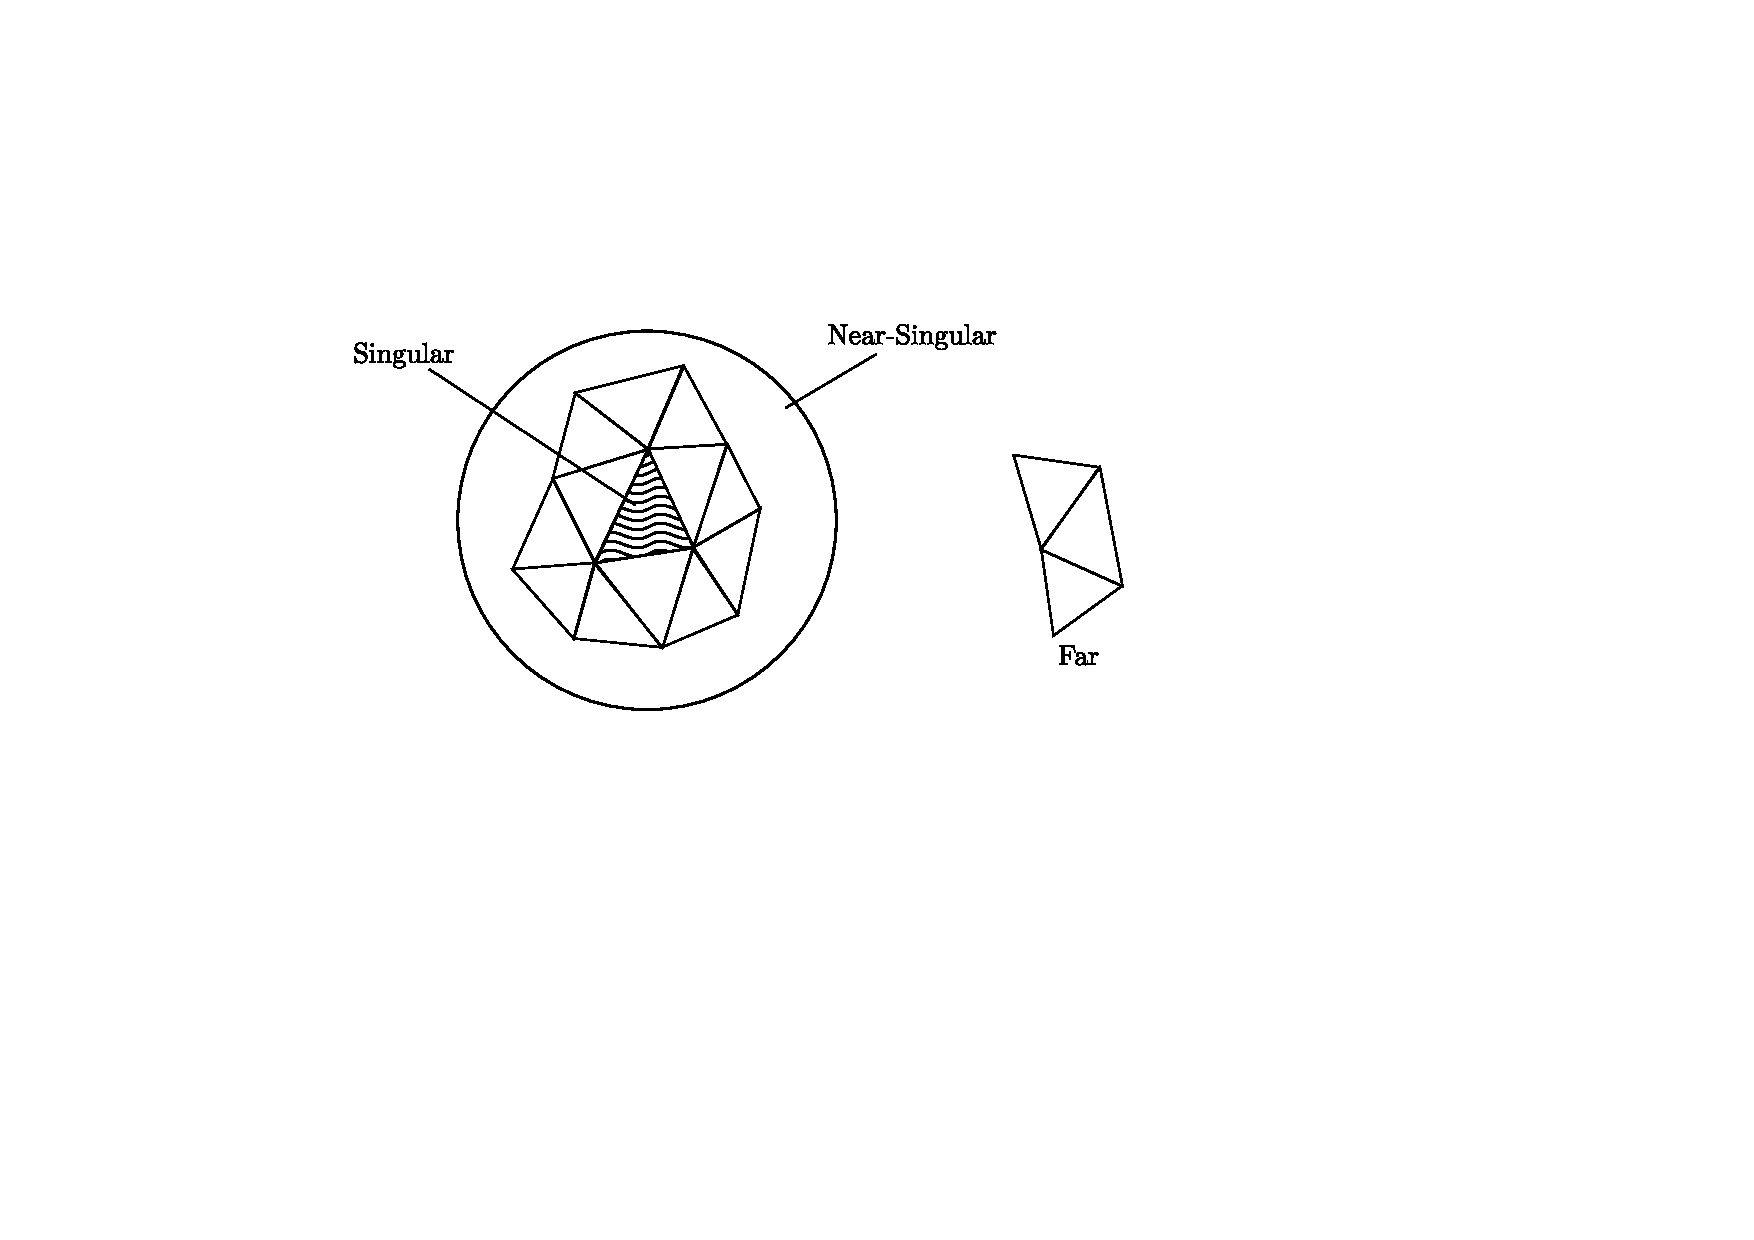
\includegraphics[width=12cm]{img/IntegrationDomain.pdf}
	\caption{Integration domains}
	\label{fig:integration_domain}
	\end{centering}
\end{figure}

%%%%%%%%%%%%%%%%%%%%%%%%%%%
% GAUSS QUADRATURE
%%%%%%%%%%%%%%%%%%%%%%%%%%%
\subsection{Gauss Quadrature}\label{subsubsec:quadrature}

Gaussian quadrature is an approximation to a definite integral, formed by a weighted sum of $K$ function evaluations at $K$ \emph{gauss points}, $x_k$ and \emph{gauss weights}, $w_k$ within the integration region. As a 1D example, consider the integral of a single-valued function, $f(x)$ over a line segment, $[a,b]$.

\begin{equation}
	\int_a^{b} f(x)\;\di{x} \approx \sum_{k=1}^{K} w_k f(x_k), \;\; w_k\in[0,1],\; x_k \in [a,b].
	\label{eqn:quadrature_1}
\end{equation}

This method is generalizable over $n$-dimensions, so for a multi-variate function $f(\vect{x}),\;\vect{x}\in\R^{d}$ defined in some region, $\D$, \ref{eqn:quadrature_1} changes very little, to

\begin{equation}
	\int_{\D} f(\vect{x})\;\di{\vect{x}} \approx \sum_{k=1}^{K} w_k f(\vect{x}_k), \;\; w_k\in[0,1],\; \vect{x}_k \in \D.
	\label{eqn:quadrature_2}
\end{equation}

For an example of this, we can look at the integrals resulting from the {\bem} formulation for the Laplace equation, given later in equations \ref{eqn:laplace_bem_G} and \ref{eqn:laplace_bem_dGdn}. In this case, $\vect{x}_i$ is a target point, and $j$ denotes a particular panel. Using a rule of the form from \ref{eqn:quadrature_2} these integrals turn into

\begin{eqnarray}
	\int_{\Gamma} G(\vect{x}_i,\vect{x}_j)\;\di{\Gamma_j} & \approx & \sum_{k=1}^{K} w_k\cdot A_j\cdot \frac{1}{|\vect{x}_i-\vect{x}_k|},\;\;\vect{x}_k \in \Gamma_j, \\ 
	\int_{\Gamma} \partiald{G(\vect{x}_i,\vect{x}_j)}{\nhat_j}\;\di{\Gamma_j} & \approx & \sum_{k=1}^{K}w_k\cdot A_j\cdot \frac{d\vect{x}\cdot\nhat_j}{|\vect{x}_i-\vect{x}_k|^{3}},\;\;\vect{x}_k \in \Gamma_j,
\end{eqnarray}

\noindent
where $w_k$ are area-normalized Gauss quadrature weights and $A_j$ is the area of $\Gamma_j$. The accuracy of the integral can be controlled by changing the number of quadrature points used, $K$. Common values for far integrals include $K=3,4$, while near-singular, many more Gauss points, for instance $K=19, 25$ may be necessary. It is worth noting here that both integrals are now expressed in terms of repeated evaluations of $1/r$ and $\nabla (1 / r)\cdot\nhat_j$, making them suitable for use with an {\fmm} and enabling us to speedup the solution to the linear system. %  It is this property that we use to enable the speedup of the solution to our system using {\fmm} and treecodes.

Each quadrature point is expressed in terms of a set of normalized co-efficients and an area-normalized weight. Given a set of co-efficients $\xi_1,\;\xi_2,\;\xi_3$, we can express the associated quadrature point, $(x_p,y_p,z_p)^{T}$ on a triangle defined by 3 vertices, $(x_1,y_1,z_1),\;(x_2,y_2,z_2),\;(x_3,y_3,z_3)$ in the following way:

\begin{equation}
\left (
	\begin{array}{c}
	x_p \\
	y_p \\
	z_p
	\end{array}
	\right ) = \left ( \begin{array}{ccc}
				x_1 & x_2 & x_3 \\
				y_1 & y_2 & y_3 \\
				z_1 & z_2 & z_3
				\end{array} \right )	\times \left ( \begin{array}{c}
													\xi_1 \\
													\xi_2 \\
													\xi_3
												   \end{array}\right ).
\end{equation}

This allows us to use the same sets of quadrature co-efficients for every integral without any changes. We use both standard low-order quadrature rules, with $k=3,4,7$, but also have much higher-precision options available for near-singular integrals. Our default rule for near-singular integrals uses $k=25$, while even higher precisions are available, for instance $k=79$.

Example co-efficients for $K=3$ for a triangular panel are given in table \ref{tab:gauss_weights_k3}.

\begin{table}[h]
\begin{center}
\begin{tabular}{c|cccc}
 $k$ & $\xi_1^{k}$ & $\xi_2^{k}$ & $\xi_3^{k}$ & $w_k$ \\
  & & & & \\
 1 & 1/2 & 1/2 & 0 & 1/3 \\
  & & & & \\
 2 & 0 & 1/2 & 1/2 & 1/3 \\
  & & & & \\
 3 & 1/2 & 0 & 1/2 & 1/3
 
\end{tabular}
\end{center}
\caption{Co-efficients and weights for Gauss integration over a triangular panel, $K=3$}
\label{tab:gauss_weights_k3}
\end{table}%

%[[[ ADD EXAMPLES OF CO-EFFICIENTS AND WEIGHTS? ]]]

%%%%%%%%%%%%%%%%%%%%%%%%%%%
% SEMI ANALYTICAL INTEGRALS
%%%%%%%%%%%%%%%%%%%%%%%%%%%
\subsection{Semi-Analytical}\label{subsubsec:semi_analytical}

The first approach for singular and near-singular integrals, will deal with the case that the function being integrated is (excluding constants) only a function of $r$, that is, $f = f(r)$, and $\int_a^{b} f(r)\;\di{r}$ can be computed analytically.

The technique we will describe relies on the fact that the integral over a polygon can be decomposed into a \emph{signed summation} of the triangles resulting from the projection of the target point onto the polygon plane, denoted $P$, and two of the polygon vertices. In this way

\begin{equation}
	\int_\Gamma f(r)\;\di{r} = \sum_{i=0}^{\# \text{vertices}} s_i \int_{PV_iV_{i+1}} f(r)\;\di{r},
\end{equation}

\noindent
where $s_i$ is the signing term, given by $1$ if $v_iv_{i+1}$ is clockwise from the target point, and $-1$ otherwise. This composition is shown in figure \ref{fig:semi_analytical_decomposition}.


\begin{figure}[ht]
\begin{center}
	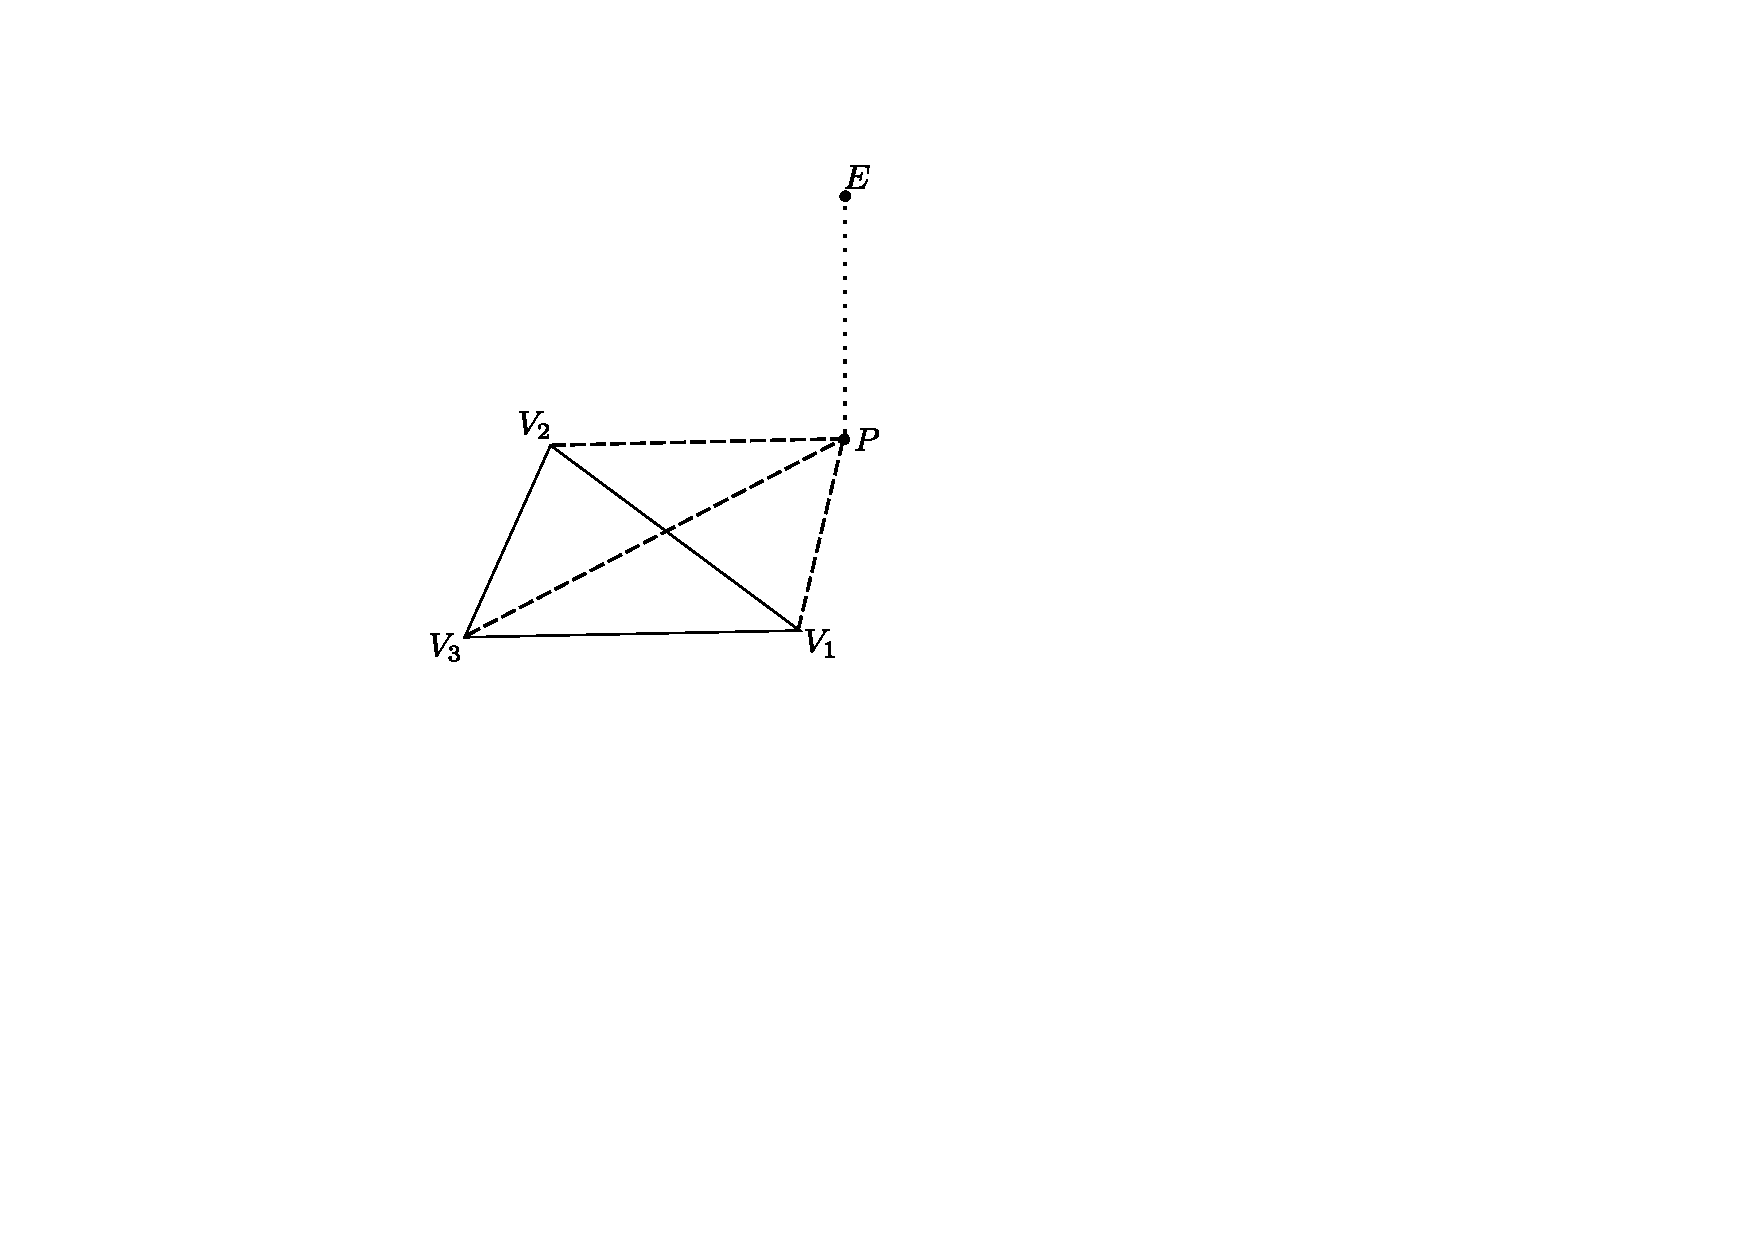
\includegraphics[width=8cm]{img/SemiAnalyticalDecomposition.pdf}
	\caption{Integral decomposition into triangles}
	\label{fig:semi_analytical_decomposition}
	\end{center}
\end{figure}


\begin{figure}[ht]
\begin{center}
	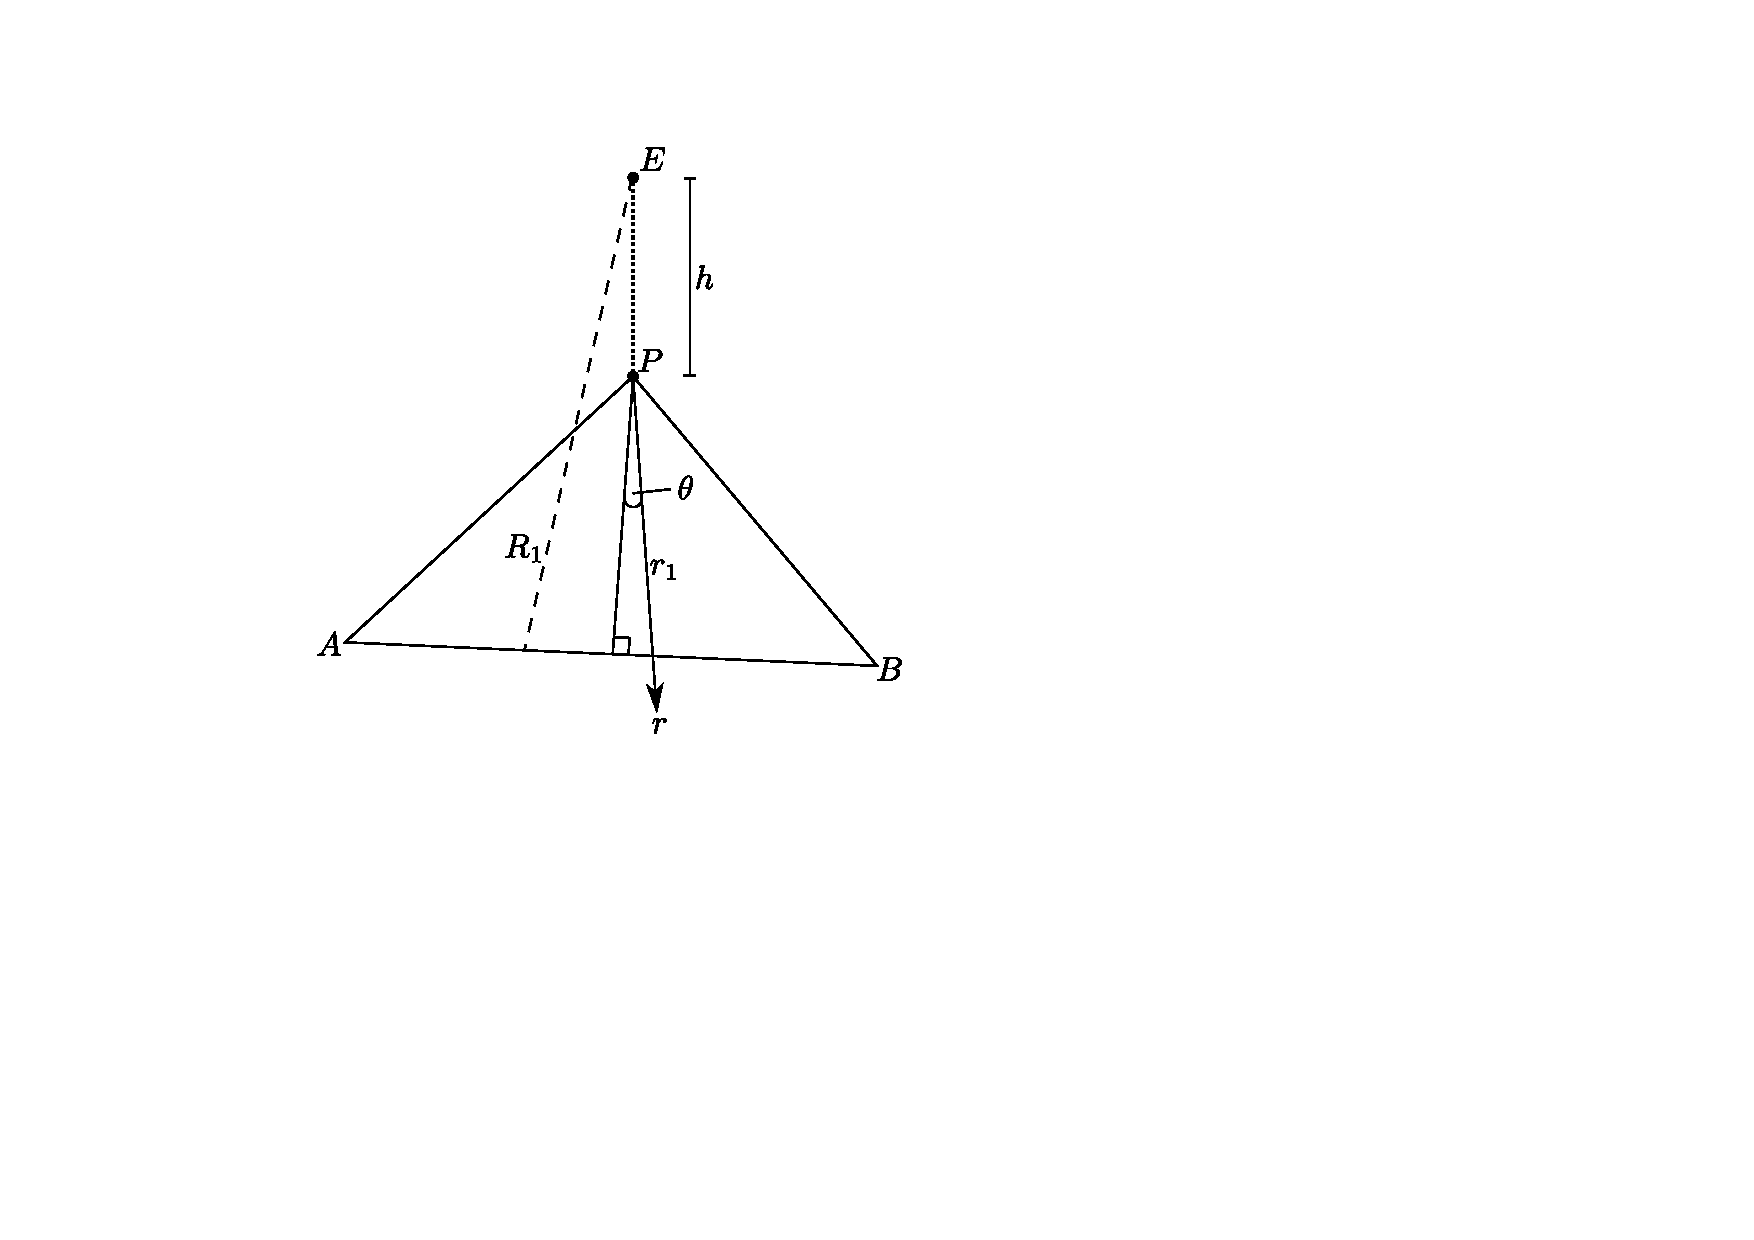
\includegraphics[width=8cm]{img/SemiAnalyticalIntegral.pdf}
	\caption{Individual triangular integral setup}
	\label{fig:semi_analytical_integral}
\end{center}
\end{figure}

For each of the individual integrals, we set up the integration domain, figure \ref{fig:semi_analytical_integral}, noting that $R = \sqrt{r^{2}+h^{2}}$ and then
\begin{eqnarray}
	\frac{\text{d}R}{\text{d}r} & = & \frac{r}{\sqrt{r^{2}+h^{2}}} \nonumber \\
	\text{d}R & = & \frac{r}{R}\;\text{d}r \nonumber \\
	R\;\text{d}R & = & r\;\text{d}r \nonumber
\end{eqnarray}

If we denote the integral over this triangle by $I$, then we can now write

\begin{eqnarray}
	I & = & \int_{\theta_1}^{\theta_2}\int_0^{r_1(\theta)} f(r)\cdot r\;\di{r}\;\di{\theta} \nonumber \\
	    \label{eqn:inner_1} & = & \int_{\theta_1}^{\theta_2}\int_h^{R_1(\theta)} f(R)\cdot R\;\di{R}\;\di{\theta}.
\end{eqnarray}

Similarly, to find the integral of the derivative of $f(r)$ in a direction, $\partialdi{I}{x_i}$, we can perform

\begin{equation}
	\label{eqn:inner_2}
	\partiald{I}{x_i} = \partiald{}{x_i} \int_{\theta_1}^{\theta_2} \int_h^{R_1(\theta)}f(R)\cdot R \;\di{R}\;\di{\theta}
\end{equation}

The inner integrals in equations \ref{eqn:inner_1} and \ref{eqn:inner_2} over $R$ will be performed analytically, then the outer integral over $\theta$ will be done using gaussian quadrature. As a first example, we look at the Green's function for Laplace's equation, $f(R) = 1 / R$
\begin{eqnarray}
	\int_h^{R_1(\theta)} f(R)\cdot R\;\di{R} & = & \int_h^{R_1(\theta)}1\;\di{R} \nonumber \\
	& = & R_1(\theta) - h. \nonumber \\
	\partiald{}{\nhat}\int_h^{R_1(\theta)} f(R)\cdot R\;\di{R} & = & \partiald{R_1(\theta)}{\nhat} -\partiald{h}{\nhat} \nonumber \\ 
	& = & \frac{z}{R(\theta)}-\text{sign}(z) \nonumber
\end{eqnarray}

Next, we look at the Yukawa equation, $f(R) = \exp(-kR) / R$

\begin{eqnarray}
	\int_h^{R_1(\theta)} f(R)\cdot R\;\di{R} & = & \int_h^{R_1(\theta)}e^{-kR}\;\di{R} \nonumber \\
	& = & -\frac{1}{k}\left [ e^{-kR_1(\theta)} - e^{-kh}\right ] \nonumber \\
	\partiald{}{\nhat}\int_h^{R_1(\theta)} f(R)\cdot R\;\di{R} & = & \frac{z\cdot e^{-kR(\theta)}}{R(\theta)} - e^{-kR(\theta)}\cdot\text{sign}(z) \nonumber
\end{eqnarray}

Now that we have the singular integrals available for Laplace and modified-Helmholtz, it is time to tackle the integrals that this semi-analytical method is unsuitable for -- the Green's functions for the Stokes equation. This will be handled with an analytical expression.

%%%%%%%%%%%%%%%%%%%%%%%%%%%
% ANALYTICAL
%%%%%%%%%%%%%%%%%%%%%%%%%%%
\subsection{Analytical}\label{subsubsec:analytical}

For functions that cannot be expressed purely in terms of $f(r)$, we need a different approach to the semi-analytical one described in \ref{subsubsec:semi_analytical}. In these cases, we have chosen to use a purely analytical method, described by S. Fata for both Laplace \cite{fata2009} and linear elasticity \cite{fata2011}, and trivially adaptable for the Stokes equations.

We begin with a triangle described by its 3 vertices, $\vect{y}_1, \vect{y}_2$ and $\vect{y}_3$, defined in a clockwise direction. In this way, the 3 line components of the triangle are described in terms of the vertices, with $L_1 = [\vect{y}_1, \vect{y}_2]$, $L_2 = [\vect{y}_2, \vect{y}_3]$, $L_3 = [\vect{y}_3, \vect{y}_1]$. The plane in which the triangle lies is denoted by $E_q$. Next, we compute an orthonormal companion reference $\{\vect{e}_1, \vect{e}_2, \vect{e}_3 \}$, designed so that $\vect{e}_1$ is parallel to $L_1$, and $\vect{e}_3$ is perpendicular to the edges of the triangle and points in the direction of the outward normal. The plane spanned by $\vect{e}_1$ and $\vect{e}_2$ is referred to by $P_{E_q}$. Thus, we introduce a new co-ordinate system, $\vect{x}; \xi, \zeta, \eta$ that is associated with $E_q$, shown in figure \ref{fig:fata_local_coordinate}.

\begin{figure}[hc]
\begin{centering}
	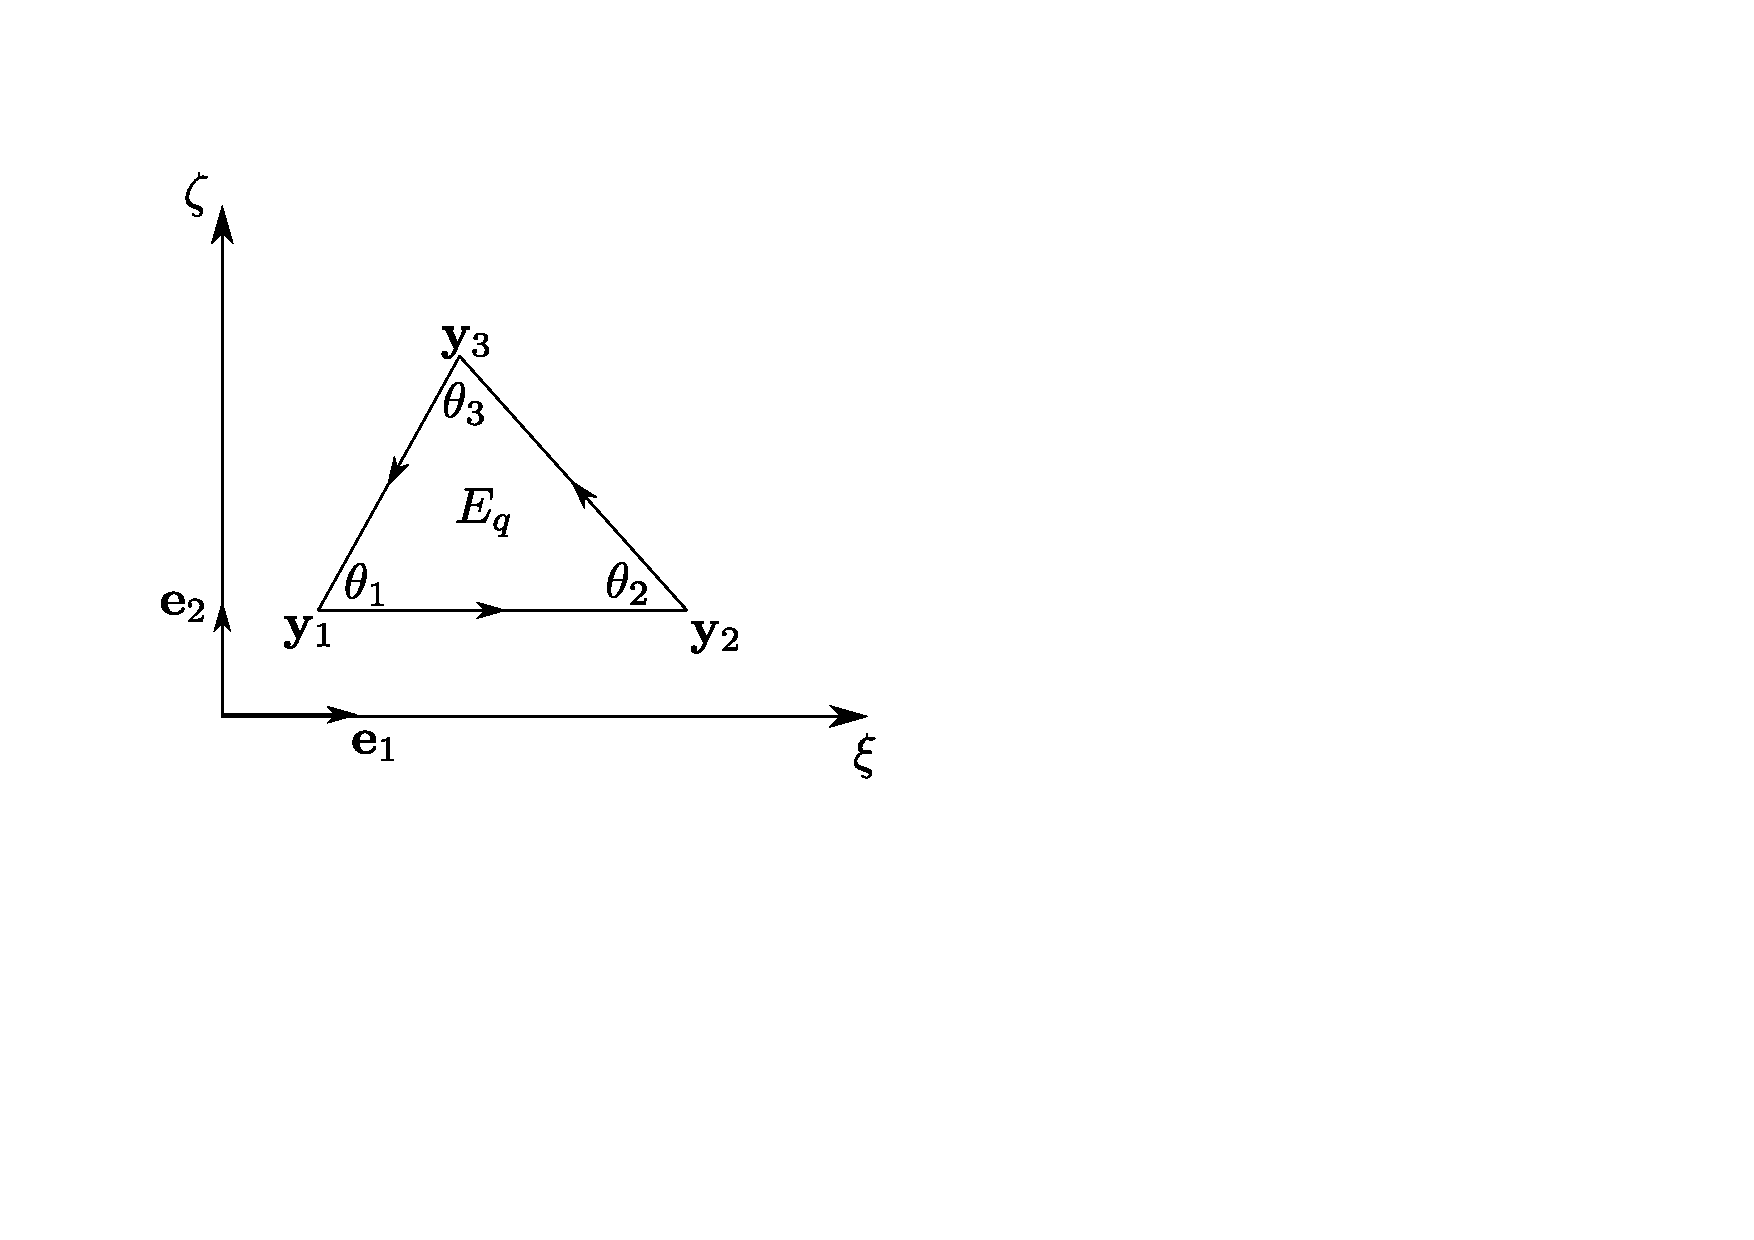
\includegraphics[width=10cm]{img/FataGeometry.pdf}
	\caption{Local co-ordinate system for analytical integrals}
	\label{fig:fata_local_coordinate}
\end{centering}
\end{figure}

Using this co-ordinate system, we can describe important quantities which are used to describe our integrals in the forms shown in equations \ref{eqn:generic_int1} and \ref{eqn:generic_int2}.
\begin{eqnarray*}
	\vect{r} & = & \vect{y}-\vect{x} = \xi\vect{e}_1 + \zeta\vect{e}_2 + \eta\vect{e}_3 \\ 
	r & = & ||\vect{y}-\vect{x}|| = \sqrt{\xi^{2} + \zeta^{2} + \eta^{2}},
\end{eqnarray*}
%
%\noindent
%that we can use to describe our integrals in the following forms:

\begin{eqnarray}
	\int_{\Gamma_j} G(\vect{x},\vect{y}) \di{\Gamma_j} & = & \frac{1}{4\pi}I_1 \label{eqn:generic_int1}\\
	& & \nonumber \\
	\int_{\Gamma_j} \partiald{G_j(\vect{x})}{\nhat} \di{\Gamma_j} & = & -\frac{\eta}{4\pi}I_3, \label{eqn:generic_int2}
\end{eqnarray}

\noindent
where the generic integrals $I_1,\; I_3$ refer to:

\begin{equation}
	I_1 = \int_{E_q} \frac{1}{r} \di{s}, \;\;\;I_3 = \int_{E_q} \frac{1}{r^{3}} \di{s}
\end{equation}

To express these generic integrals, we must define some more quantities over the panel. First, $\theta_i \in (0,\pi)$ is the inclusion angle at vertex $i$, such that $\theta_1 + \theta_2 + \theta_3 = \pi$, next we define $\alpha_1 = 0,\;\alpha_2 = \pi-\theta_2,\;\alpha_3 = \pi + \theta_1$. Using these values of $\theta_i$ and $\alpha_i$ we can constuct a set of 3 local orthonormal bases centred at the origin, given by $\{\vect{e}_{p_i}, \vect{e}_{q_i}, \vect{e}_3\}$, such that $\vect{e}_{p_i}$ is parallel to the previously defined line $L_i$. This gives us local coordinated systems, denoted by $\{p_i, q_i, \eta\}$ that are associated with each edge of the triangle. In this form, we have
\begin{equation}
	p_i = \xi\cos\alpha_i + \zeta\sin\alpha_i, \;\;\;\;q_i = -\xi\sin\alpha_i + \zeta\cos\alpha_i.
\end{equation}

More local coordinate systems can be formed from this construction, $\utilde{\vect{x}} = (p_i, q_i)$ defined for each of the sides of the triangle, allowing us to write a local coordinate $(p_i^{j},q_i^{j},\eta)$ in terms of a basis $\{\vect{e}_{p_i}, \vect{e}_{q_i}, \vect{e}_3\}$. The distance $\rho_j$ between a vertex, $\vect{y}_i$ and a source point, $\vect{x}$ can now be written as
\begin{equation}
	\rho_j = \sqrt{(p_i^{j})^{2} + (q_i^{j})^{2}+\eta^{2}}.
\end{equation}

To make the following equations simpler, we define
\begin{equation}
	\tilde{\rho}_1 = \rho_1-\rho_2,\;\;\tilde{\rho}_2 = \rho_2 - \rho_3,\;\;\tilde{\rho_3} = \rho_3-\rho_1,\;\;d_i = (q_i)^{2} + \eta^{2},\;\;i = 1,2,3.
\end{equation}

More quantities are now defined over each side, $L_i$,

\begin{equation}
	\gamma_i(\vect{x}) = \arctan\left ( \frac{-2p^{i}_iq_i\eta\rho_i}{(q_i)^{2}(\rho_i)^{2}-(p_i^{i})^{2}\eta^{2}} \right ) - \arctan\left ( \frac{-2p_i^{i+1}q_i\eta\rho_{i+1}}{(q_i)^{2}(\rho_{i+1})^{2}-(p_i^{i+1})^{2}\eta^{2}} \right )
\end{equation}
\begin{eqnarray}
	\chi_i(\vect{x}) & = & \ln(p_i^{i}+\rho_i) - \ln(p_i^{i+1}+\rho_{i+1}), \\ 
	\delta_i(\vect{x}) & = & \frac{p_i^{i}}{\rho_i} - \frac{p_i^{i+1}}{\rho_{i+1}}, \\
	\L_i(\vect{x}) & = & \frac{1}{\rho_i} - \frac{1}{\rho_{i+1}}.
\end{eqnarray}

Discarding all explicit dependancies on $\vect{x}$ for brevity's sake, we define the last couple of quantities needed, $\theta_0(\vect{x})$, dependant on the location of the center of the source panel and $\theta(\vect{x})$.

\begin{equation}
	\theta_0(\vect{x}) = 
	\begin{cases}
		0 & \text{if}\; \utilde{\vect{x}} \in P_{E_q}\setminus \bar{E_q} \\
		\pi & \text{if}\; \utilde{\vect{x}} \in \L_q\setminus\{ \vect{y}_1, \vect{y}_2, \vect{y}_3 \} \\
		2\pi & \text{if}\; \utilde{\vect{x}} \in E_q \\
		\theta_i & \text{if}\; \utilde{\vect{x}} = \vect{y}_i, \;\; i=1,2,3
	\end{cases}
\end{equation}

\begin{equation}
	\theta(\vect{x}) = \frac{1}{2}\sum_{i=1}^{3}\gamma_i(\vect{x}) + \sign(\eta)\theta_0(\vect{x})	
\end{equation}

This allows us to finally define $I_1$ and $I_3$ as:

\begin{eqnarray}
	I_1 & = & \sum_{i=1}^{3} q_i\chi_i(\vect{x}) - \eta\theta(\vect{x}) \\ 
	I_3 & = & \frac{1}{\eta} \theta(\vect{x}),
\end{eqnarray}

\noindent
allowing us to compute the desired integrals.

This work on analytical integrals for potential problems was later extended to linear elasticity integrals \cite{fata2011}, which can then be devolved into Stokes kernels by setting the poisson ratio, $\nu = 1 / 2$. By using the same quantities over the triangle as from the potential integrals, we can express these Stokes integrals in a similar fashion

\begin{eqnarray}
	U(\vect{x},\vect{y}) & = & \frac{1}{8\pi\mu}\left (\frac{\vect{I}}{r} + \frac{(\vect{x}-\vect{y})\otimes(\vect{x}-\vect{y})}{r^{3}}\right ) = \frac{1}{8\pi\mu}I_U\\ 
	& & \nonumber \\
	T(\vect{x},\vect{y}) & = & -\frac{3}{4\pi} \left (\frac{(\vect{x}-\vect{y})\otimes(\vect{x}-\vect{y})(\vect{x}-\vect{y})\cdot\nhat}{r^{5}} \right ) = -\frac{3}{4\pi}I_T
\end{eqnarray}

With $I_U$ and $I_T$ defined in terms of more generic integrals

\begin{equation}
	\begin{multlined}
	I_U = (I_1 + I_3^{\xi\xi})\dyad{\e_1}{\e_1} + I_3^{\xi\zeta}\dyad{\e_1}{\e_2} + \eta I_3^{\xi}\dyad{\e_1}{\e_3} \\
	+ I_3^{\xi\zeta}\dyad{\e_1}{\e_2} + (I_1 + I_3^{\zeta\zeta})\dyad{\e_2}{\e_2} + \eta I_3^{\zeta}\dyad{\e_2}{\e_3} \\
	+ \eta I_3^{\xi}\dyad{\e_1}{\e_3} + \eta I_3^{\xi}\dyad{\e_2}{\e_3} + (I_1 + \eta^{2}I_3)\dyad{\e_3}{\e_3}
	\end{multlined}
\end{equation}

\begin{equation}
	\begin{multlined}
	I_T = -3\eta I_5^{\xi\xi}\dyad{\e_1}{\e_1} - 3\eta I_5^{\xi\zeta}\dyad{\e_1}{\e_2} - 3\eta^{2}I_5^{\xi}\dyad{\e_1}{\e_3} \\
	-3\eta I_5^{\xi\zeta}\dyad{\e_1}{\e_2} -3\eta I_5^{\zeta\zeta}\dyad{\e_2}{\e_2} -3\eta^{2}I_5^{\zeta}\dyad{\e_2}{\e_3} \\
	-3\eta^{2}I_5^{\xi}\dyad{\e_1}{\e_3} -3\eta^{2}I_5^{\zeta}\dyad{\e_2}{\e_3} -3\eta^{2}I_5\dyad{\e_3}{\e_3}
	\end{multlined}
\end{equation}
where the new generic integrals are defined as:

\begin{eqnarray*}
	I_5 & = & \frac{1}{3\eta^{2}}\sum_{i=1}^{3}\frac{q_i}{d_i}\delta_i(\vect{x}) + \frac{1}{3\eta^{3}}\theta(\vect{x}) \\
	I_3^{\xi} & = & \sum_{i=1}^{3} \chi_i(\vect{x})\sin\alpha_i,\;\;\;\;I_3^{\zeta} = -\sum_{i=1}^{3} \chi_i(\vect{x})\cos\alpha_i \\
	I_5^{\xi} & = & \frac{1}{3}\sum_{i=1}^{3}\frac{\delta_i(\vect{x})}{d_i}\sin\alpha_i,\;\;\;\;I_5^{\zeta} = -\frac{1}{3}\sum_{i=1}^{3}\frac{\delta_i(\vect{x})}{d_i}\cos\alpha_i \\
	I_5^{\xi\xi} & = & -\frac{1}{3}\sum_{i=1}^{3}\left ( \L_i(\vect{x})\cos\alpha_i + \frac{q_i}{d_i}\delta_i(\vect{x})\sin\alpha_i \right )\sin\alpha_i + \frac{1}{3\eta}\theta(\vect{x}) \\ 
	I_5^{\zeta\zeta} & = & \frac{1}{3}\sum_{i=1}^{3}\left ( \L_i(\vect{x})\sin\alpha_i + \frac{q_i}{d_i}\delta_i(\vect{x})\cos\alpha_i \right )\cos\alpha_i + \frac{1}{3\eta}\theta(\vect{x}) \\
	I_5^{\xi\zeta} & = & \frac{1}{3}\sum_{i=1}^{3}\left ( \L_i(\vect{x})\sin\alpha_i + \frac{q_i}{d_i}\delta_i(\vect{x})\cos\alpha_i \right )\sin\alpha_i
\end{eqnarray*}

Finally, we have all the integration tools in order to evaluate integral expressions over the entire domain. We can now evaluate $A\vect{x}$ in each {\gmres} iteration for all the kernels we will consider, and so we can concentrate on the linear solver itself.

%%%%% RELAXATION STRATEGIES
\section{Relaxation Strategies}\label{subsec:relaxation}

All testing results presented in this thesis are obtained using relaxation strategies during our {\gmres} / {\fgmres} iterations, and are the first such work for {\fmmbem} applications. For each iteration $k$ of the solver, we define an accuracy, $\eta_{k}$ that must be fulfilled by our {\fmm}-accelerated matvec in order to continue converging. We have chosen to concentrate on the following definition for $\eta_{k}$, given by \cite{bourasfraysse2005}. 

\begin{equation} 
	\eta_{k} = \frac{\epsilon_{\text{global}}}{r_{k}},
%	\eta_{k} & = & r_{k}.
\end{equation}

\noindent
where $\epsilon_{\text{global}}$ is the desired tolerance of the solution, and $r_k$ is the residual at iteration $k$.

Given these accuracies, we need some way of imposing them on our fast method. Given that the error from said method, $\epsilon_{\text{fast}} = \epsilon_{\text{fast}}(\theta_{\text{MAC}}, p)$, we choose to modify only one parameter, holding $\theta_{\text{MAC}}$ constant, and only modifying $p$.

As an example, we choose spherical harmonics kernels for the Laplace Green's function. From \cite{GreengardRokhlin1987} we can express a given term in the multipole expansion, $M^{m}_{n}$ from source points $(\rho_{i}, \alpha_{i}, \beta_{i})$ as

\begin{equation}\label{eqn:multipole}
	M^{m}_{n} = \sum_{i=1}^{N} q_{i}\cdot\rho_{i}^{n}\cdot Y^{m}_{n}(\alpha_{i}, \beta_{i}),
\end{equation}

\noindent
and the error incurred from this approximation, for series truncation $p > 1$ at a point, $P = P(r, \theta, \phi)$, 

\begin{equation}\label{eqn:multipole_error}
	\left | \phi(P) - \sum_{n=0}^{p}\sum_{m=-n}^{n}\frac{M^{m}_{n}}{r^{n+1}}\cdot Y^{m}_{n}(\theta, \phi) \right | \leq \frac{\sum_{i=1}^{N}q_{i}}{r-a}\left ( \frac{a}{r} \right )^{p+1},
\end{equation}

\noindent
where $a$ is the size of the cluster and $r$ is the distance between the multipole center and the target particle. Similar bounds are derived \cite{greengard1987} for all of the translation and evaluation operators. Using the nature of the octree space decomposition, we can form the following expression for the number of terms needed for a given accuracy,

\begin{equation}\label{eqn:fmm_p}
	p \sim \lceil -\log_{2}(\epsilon) \rceil.
\end{equation}

While in practice this presents a very loose error bound, often over-approximating the value of $p$ needed for a desired accuracy, the fact that it requires no knowledge of the tree or interactions between boxes is advantageous, and allows us to choose a new $p$ in $\O{1}$ time.

% -- a better approach is needed. We currently have 2 main options for this new approach, summarised below

%\begin{itemize}
%
%	\item \emph{Tabulate errors and $p$ necessary} -- This could potentially be both fast and provide very good estimates of $p$. However, the error incurred by a given truncation point differs based on the layout of the source particles, and so a table that works very well for uniform distributions may give wrong $p$ values for non-uniform distributions (such as those found in {\bem} problems)
%	
%	\item \emph{Use full error equation} -- This approach should provide very good estimates, but will be comparatively more expensive that the tabular approach. Estimates could also be high due to needing to take into account the error incurred at the highest levels of the tree. This also requires a lot more information to calculate, and will likely involve an iterative method to determine the correct value of $p$.
%	
%\end{itemize}

%%%%% PRECONDTIONERS
\section{Preconditioners}\label{subsec:preconditioners}

In this work we will make use of a small number of fairly simple preconditioners, implemented for each of our test problems. In each case, for the right-preconditioned {\gmres} we are providing a solution to the system
\begin{equation}
	Mz_j = v_j,
\end{equation}

\noindent
where $M$ is some approximation of $A$, such that solving for $z_j$ is cheaper than actually solving $Az_j = v_j$, or $M^{-1}$ is easily computable.

The first, and most basic preconditioner that can be used is a diagonal preconditioner, where
\begin{equation}
	M = \text{diag}(A).
\end{equation}

With this form of $M$, $M^{-1}$ becomes $M^{-1}_{ii} = (A_{ii})^{-1}$. For the Laplace equation, $(A_ii)^{-1}$ is simply $1 / A_ii$, while for Stokes problems, where $A_{ii} \in \R^{3\times 3}$, each element of $M^{-1}$ is the $3\times3$ matrix inverse of $A_{ii}$. Note that this is a \emph{constant} preconditioner with no inner solve needed, and thus can be used in both {\gmres} and {\fgmres} solvers.

Next, we look at 2 preconditioners that are made possible by the {\fmm}'s decomposition of space. First is a block-diagonal form, shown in \cite{Liu2009} where $M$ is a sparse matrix taking into account only particle-particle interactions within a leaf of the {\fmm}'s tree hierarchy. This takes into account only the closest interactions between panels. We denote this sparse matrix as $A_{\text{leaf}}$, and precompute at the start of all calculations. Each block of this matrix is independent, and so we could explicitly compute the inverse (using {\blas} or similar). However, we do not do this currently, and instead solve $A_{\text{block}}z_j = v_j$ using an inner {\gmres} solver. Due to the inner solve, this preconditioner is considered to be \emph{flexible}, and so {\fgmres} must be used as the outer solver. In the matrix form shown below, $A_i$ denotes the block matrix formed by interactions within leaf $i$ of the tree.

\begin{equation} A_{\text{leaf}} = 
\left(\begin{array}{ccccc}
	A_1 &   &   &   &   \\
	  & A_2 &   &   &   \\
	  &   & A_3 &   &   \\
	  &   &   & \ddots &   \\
	  &   &   &   & A_N
\end{array}\right),\;\;\;
A_{\text{leaf}}^{-1} = 
\left(\begin{array}{ccccc}
	A_1^{-1} &   &   &   &   \\
	  & A_2^{-1} &   &   &   \\
	  &   & A_3^{-1} &   &   \\
	  &   &   & \ddots &   \\
	  &   &   &   & A_N^{-1}
\end{array}\right)
\end{equation}

In a similar vein, the third preconditioner we experiment with takes into account all close-range interactions within the {\fmm} \cite{Chailletetal2011}. This preconditioner involves only $\ptop$ interactions, and no far-field approximations of any kind. By necessity, the interactions are precomputed and stored as the sparse-matrix $A_{\text{local}}$. We are unable to efficiently compute the inverse (which is not guaranteed to be sparse), so, as with the block-diagonal preconditioner described above, we use an additional {\gmres} solver to obtain $z_j$. Again, this is a \emph{flexible} preconditioner an {\fgmres} must be used. For this case, in the notation used below, $A_{ij}$ is the block matrix formed from interactions between leaves $i$ and $j$.

\begin{equation} A_{\text{local}} = 
\left(\begin{array}{ccccc}
	A_{11} & A_{12}  & A_{13}  &   &   \\
	A_{21}  & A_{22} & A_{23}  &   &   \\
	  & A_{32} & A_{33} & A_{34}  &   \\
	  &   &   & \ddots &  \\
	  &   &   &  A_{N,N-1} & A_{NN}
\end{array}\right)
\end{equation}

This ends up being another sparse approximation to the full linear system, albeit one more dense than the block-diagonal preconditioner. Intuitively, we could expect this preconditioner to work the best in terms of reducing iteration counts as it better represents $A$, however this will come at a cost -- each inner {\gmres} will be more expensive due to the larger number of non-zeros.
